\documentclass[tikz,border=10pt]{standalone}
\usepackage{tikz}
\usepackage{listings}
\usetikzlibrary{arrows.meta, positioning}
\lstset{language=C, basicstyle=\ttfamily}

\begin{document}

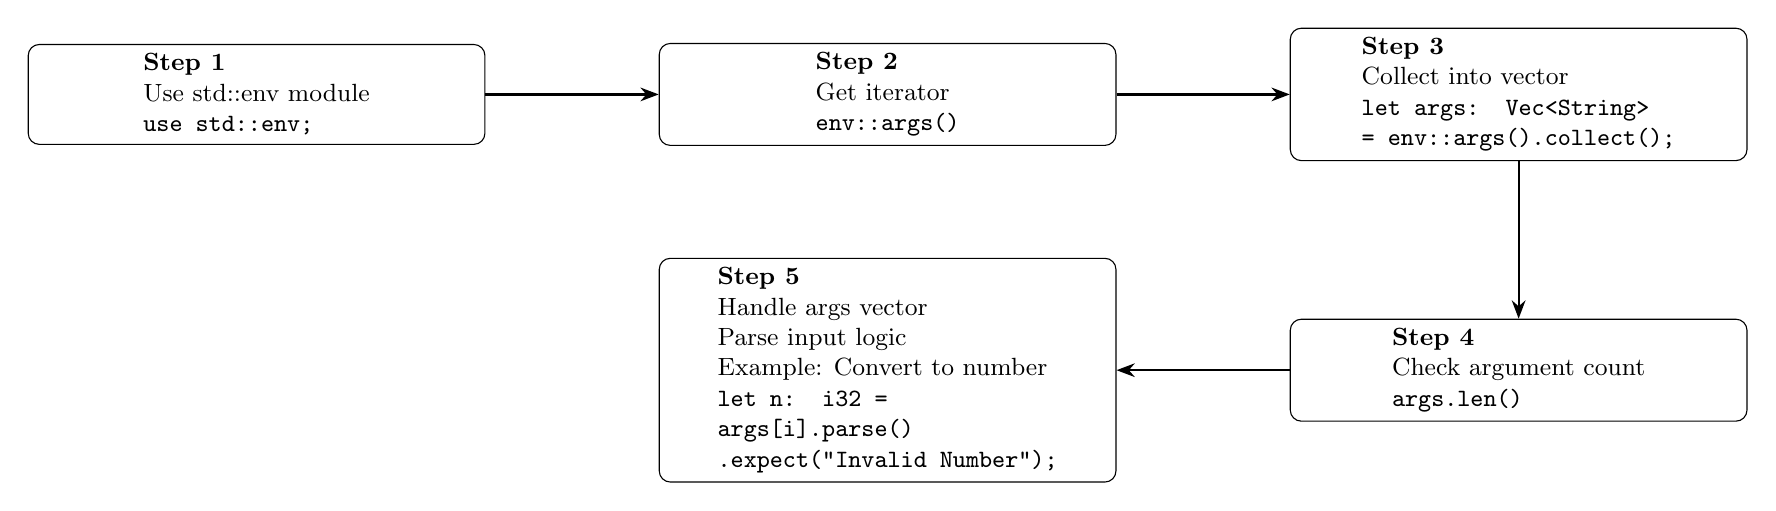
\begin{tikzpicture}[
    box/.style={
        draw,
        rounded corners,
        minimum width=5.8cm,
        minimum height=1.1cm,
        align=left,
        font=\small
    },
    arrow/.style={
        ->,
        thick,
        >=Stealth
    },
    node distance=1.6cm and 2.2cm
]

% Top row (Left → Right)
\node[box] (step1) {
\textbf{Step 1} \\
Use std::env module \\
\texttt{use std::env;}
};

\node[box] (step2) [right=of step1] {
\textbf{Step 2} \\
Get iterator \\
\texttt{env::args()}
};

\node[box] (step3) [right=of step2] {
\textbf{Step 3} \\
Collect into vector \\
\texttt{let args: Vec<String>} \\
\texttt{= env::args().collect();}
};

\node[box] (step4) [below=2cm of step3] {
\textbf{Step 4} \\
Check argument count \\
\texttt{args.len()}
};


\node[box] (step5) [left=of step4] {
\textbf{Step 5} \\
Handle args vector \\
Parse input logic \\
Example: Convert to number \\
\texttt{let n: i32 =} \\
\texttt{args[i].parse()} \\
\texttt{.expect("Invalid Number");}
};

% Arrows (snake style)
\draw[arrow] (step1) -- (step2);
\draw[arrow] (step2) -- (step3);
\draw[arrow] (step3) -- (step4);
\draw[arrow] (step4) -- (step5);

\end{tikzpicture}

\end{document}
